\section*{Materials and Methods}

Statistical alignment is typically performed using pairwise hidden Markov models (pair-HMMs), which have the ability to rigorously model molecular sequence evolution \citembe{bradley2007transducers}.
Pair-HMMs are computational machines with two output tapes. Pair-HMMs contain a finite number of states---typically labeled match, insert, and delete---that emit symbols (nucleotides or amino acids) to one or both tapes.
Each tape represents a sequence and a path through a pair-HMM is a possible pairwise alignment.
Conceptually, these machines generate two sequences ($\text{X}$ and $\text{Y}$) from an unknown ancestor and can calculate the probability that two sequences are related, represented by $P(\text{X}, \text{Y})$ \citembe{yoon_2009_hmm}.

A limitation of pair-HMMs is that they only model the evolution of two related sequences from an unknown ancestor.
Finite-state transducers (FSTs) have similar benefits to pair-HMMs with the additional feature that can model the generation of a descendant sequence given an ancestral one.
FSTs consume symbols from an input tape and emit symbols to an output tape.
Properly weighted, an FST can calculate the probability that a descendant sequence, $\text{Y}$, evolved from an ancestral sequence, $\text{X}$, represented by $P(\text{Y} | \text{X})$.
Furthermore, well-established algorithms for combining FSTs in different ways allow the design of complex models by combining simpler FSTs \citembe{bradley2007transducers}.
A powerful and versatile algorithm for comparative sequence analysis is composition, which consists of sending the output of one FST into the input of a second FST.
COATi uses composition to derive a statistical alignment model from the combination of smaller FSTs, each representing a specific process.

COATi implements the pairwise alignment of a potentially lower-quality sequence against a high-quality sequence as a path through the Evolution FST (Fig.\ \ref{fig:evolution-fst}) \citep[c.f.][]{holmes2001evolutionary}.
Here, COATi treats the high-quality (reference) sequence as the ``ancestor'' and the potentially lower-quality sequence as the ``descendant''.
This FST is the result of composing a substitution FST that encodes a codon model (Fig.\ \ref{fig:evolution-fst}-a) and an indel FST that models insertions and deletions, including frameshifts (Fig.\ \ref{fig:evolution-fst}-b).
A key innovation of this FST with respect to others is the combination of a codon substitution model with a nucleotide-based geometric indel model that allows gaps to occur at any position.

Composing both sequences with the Evolution FST results in the transducer of all possible alignments.
Any path through this FST represents a pairwise alignment, while the shortest path (by weight) corresponds to the best alignment.
All FST operations in COATi, including model development, composition, search for the shortest path, and other optimization algorithms, are performed using the C++ openFST library \citembe{allauzen2007openfst}.
However, the Evolution FST has a large state space to keep track of codon substitution rates when codons might be interspersed with indel events. This additional state space increases the computational complexity of the alignment algorithm.

\begin{figure}[h!]
\centering
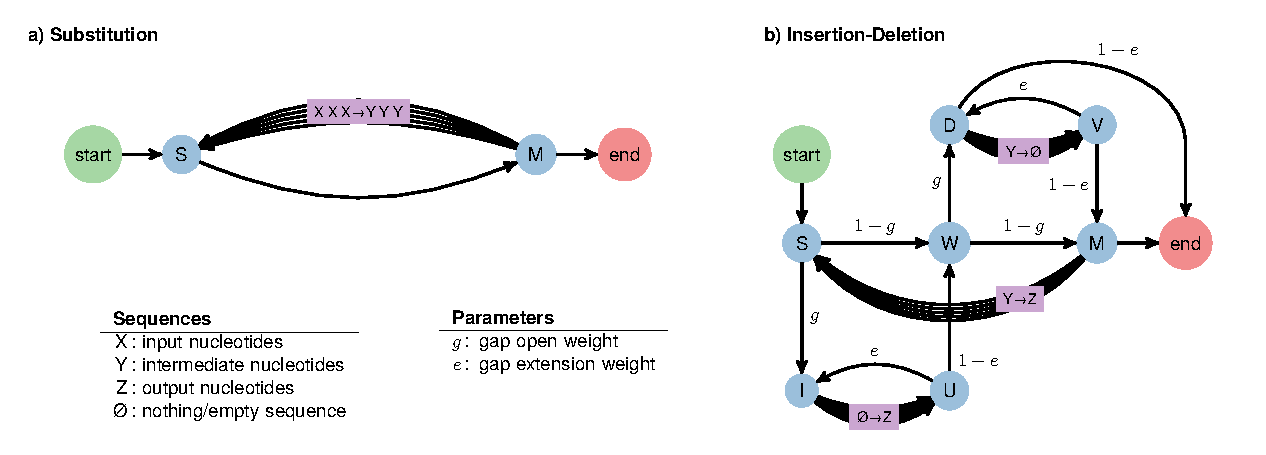
\includegraphics[width=\textwidth]{fig-evolution-fst.pdf}
\par
\caption{The Evolution FST is assembled by composing a substitution FST and an indel FST.
Each node represents a state in an FST while arcs display possible transitions between states (and their weights). Unlabeled arcs have weights of 1.
(a) The substitution FST encodes a $61 \times 61 $ codon substitution model with 3721 arcs from M to S. These arcs consume three nucleotides from the input tape and emit three nucleotides to the output tape. The weight of each arc is a conditional probability derived from a codon substitution model.
(b) The indel FST allows for insertions (I to U) and deletions (D to V). Insertion arcs are weighted according to the codon model's stationary distribution of nucleotides, and deletion arcs have a weight of 1. On top of the indel FST we add a base calling error FST (Figure S1) to model sequencing errors. Contiguous insertions and deletions are always arranged for insertions to precede deletions to limit equivalent alignments.}
\label{fig:evolution-fst}
\end{figure}

Codon substitution models are uncommon in sequence aligners, despite their extensive use in phylogenetics.
COATi implements the Muse and Gaut (\citeyear{muse_gaut_1994}) codon model (codon-triplet-mg) and the Empirical Codon Model \citembe{kosiol_ECM_2007} (codon-triplet-ecm).
It also lets the user provide a codon substitution matrix.
The default FST model (codon-triplet-mg) does not allow early stop codons in the ancestor sequence; although, it does support mutations to (early) stop codons under the assumption that these are artifacts common in low-quality data.

To reduce the runtime complexity of COATi, we have also developed an approximation of the Evolution FST that can be implemented with standard dynamic programming techniques. This approximation uses a marginal substitution model where the output nucleotides are independent of one another and only depend on the input codon and position. This produces a $\left(61 \times 3 \right) \times 4$ substitution model and eliminates the need to track dependencies between output nucleotides.

A marginal substitution model is calculated from a standard substitution model by calculating the marginal probabilities that each ancestral codon produces specific descendant nucleotides at each reading frame position.
%
Specifically, let
$P_\text{cod}\left(Y_0 \cdot Y_1 \cdot Y_2 \middle| X_0 \cdot X_1 \cdot X_2\right)$ represent transition probabilities from a standard codon model, and
%
\[
P_\text{mar}\left(Y_p = y \middle| X_0 \cdot X_1 \cdot X_2\right) =
\sum_{Y_0 \cdot Y_1 \cdot Y_2} I(Y_p = y) P_\text{cod}\left(Y_0 \cdot Y_1 \cdot Y_2 \middle| X_0 \cdot X_1 \cdot X_2\right)
\]
%
represent the marginal transition probabilities, where
$p \in \{0, 1, 2\}$ is the position of the descendant nucleotide relative to the ancestral reading frame and $I$ is an indicator function defined
%
$I(e) = \{ 1 \text{ if $e$ is true and } 0 \text{ otherwise}\}$.
%
COATi contains marginal models for both Muse and Gaut or the Empirical Codon Model, resulting in the marginal models codon-marginal-mg (default model) and codon-marginal-ecm.
These models emphasize the position in a codon where the substitution occurs, help restrict the effects of low-quality data in the descendant sequence, and allow more than one substitution per codon.
In combination with the indel model, alignment using the marginal model is implemented using dynamic programming.
